\documentclass[
	a4paper,
	oneside,
	BCOR = 10mm,
	DIV = 12,
	12pt,
	headings = normal,
]{scrartcl}

%%% Length calculations
\usepackage{calc}
%%%

%%% Support for color
\usepackage{xcolor}
\definecolor{lightblue}{HTML}{03A9F4}
\definecolor{red}{HTML}{F44336}
%%%

%%% Including graphics
\usepackage{graphicx}
%%%

%%% Font selection
\usepackage{fontspec}

\setromanfont{STIX Two Text}[
	SmallCapsFeatures = {LetterSpace = 8},
]

\setsansfont{IBM Plex Sans}[
	Scale = MatchUppercase,
]

\setmonofont{IBM Plex Mono}[
	Scale = MatchUppercase,
]
%%%

%%% Math typesetting
\usepackage{amsmath}

\usepackage{unicode-math}
\setmathfont{STIX Two Math}

\usepackage{IEEEtrantools}
%%%

%%% List settings
\usepackage{enumitem}
\setlist[enumerate]{
	label*      = {\arabic*.},
	leftmargin  = *,
	labelindent = \parindent,
	topsep      = 1\baselineskip,
	parsep      = 0\baselineskip,
	itemsep     = 1\baselineskip,
	noitemsep, % override itemsep
}

\setlist[itemize]{
	label*      = {—},
	leftmargin  = *,
	labelindent = \parindent,
	topsep      = 1\baselineskip,
	parsep      = 0\baselineskip,
	itemsep     = 1\baselineskip,
	noitemsep, % override itemsep
}

\setlist[description]{
	font        = {\rmfamily\upshape\bfseries},
	topsep      = 1\baselineskip,
	parsep      = 0\baselineskip,
	itemsep     = 0\baselineskip,
}

%%%

%%% Structural elements typesetting
\setkomafont{pagenumber}{\rmfamily\upshape}
\setkomafont{disposition}{\rmfamily\bfseries}

% Sectioning
\RedeclareSectionCommand[
	beforeskip = -1\baselineskip,
	afterskip  = 1\baselineskip,
	font       = {\normalsize\bfseries\scshape},
]{section}

\RedeclareSectionCommand[
	beforeskip = -1\baselineskip,
	afterskip  = 1\baselineskip,
	font       = {\normalsize\bfseries\itshape},
]{subsection}

\RedeclareSectionCommand[
	beforeskip = -1\baselineskip,
	afterskip  = 1\baselineskip,
	font       = {\normalsize\bfseries},
]{subsubsection}

\RedeclareSectionCommand[
	beforeskip = -1\baselineskip,
	afterskip  = -0.5em,
	font       = {\normalsize\mdseries\scshape\addfontfeatures{Letters = {UppercaseSmallCaps}}},
]{paragraph}
%%%

%%% Typographic enhancements
\usepackage{microtype}
%%%

%%% Language-specific settings
\usepackage{polyglossia}
\setmainlanguage{ukrainian}
\setotherlanguages{english}
%%%

%%% Captions
\usepackage{caption}
\usepackage{subcaption}

%\DeclareCaptionLabelFormat{closing}{#2)}
%\captionsetup[subtable]{labelformat = closing}

%\captionsetup[subfigure]{labelformat = closing}

\captionsetup[table]{
	aboveskip = 0\baselineskip,
	belowskip = 0\baselineskip,
}

\captionsetup[figure]{
	aboveskip = 1\baselineskip,
	belowskip = 0\baselineskip,
}

\captionsetup[subfigure]{
	labelformat = simple,
	labelformat = brace,
}
%%%

%%% Hyphenated ragged typesetting
\usepackage{ragged2e}
%%%

%%% Table typesetting
\usepackage{booktabs}
\usepackage{longtable}

\usepackage{multirow}

\usepackage{array}
\newcolumntype{v}[1]{>{\RaggedRight\arraybackslash\hspace{0pt}}p{#1}}
\newcolumntype{b}[1]{>{\Centering\arraybackslash\hspace{0pt}}p{#1}}
\newcolumntype{n}[1]{>{\RaggedLeft\arraybackslash\hspace{0pt}}p{#1}}
%%%

%%% Drawing
\usepackage{tikz}
\usepackage{tikzscale}
\usetikzlibrary{positioning}
\usetikzlibrary{arrows.meta} % Stealth arrow tips
%%%

%%% SI units typesetting
\usepackage{siunitx}
\sisetup{
	output-decimal-marker = {,},
	exponent-product      = {\cdot},
	inter-unit-product    = \ensuremath{{} \cdot {}},
	per-mode              = symbol,
}
%%%

%%% Framing code listings
\usepackage{tcolorbox}
\tcbuselibrary{breakable}
\tcbuselibrary{minted}
\tcbuselibrary{skins}

\newtcblisting[
	auto counter, 
	list inside, 
	number within = section,
]{listingpython}[3][]{%
	minted language = python,
	minted style    = bw,
	minted options  = {
		linenos,
		tabsize = 4,
		breaklines,
		% breakanywhere,
		fontsize = \footnotesize,
		autogobble
	},
	%
	% empty,
	sharp corners,
	colframe         = black,
	colback          = black!0,
	leftrule         = 0em,
	rightrule        = 0em,
	toprule          = 1pt, % orig = 0pt
	bottomrule       = 1pt, % orig = 0pt
	titlerule        = 0.5pt,
	colbacktitle     = black!0,
	coltitle         = black,
	toptitle         = 0.3em,
	bottomtitle      = 0.1em,
	borderline north = {1pt}{0pt}{black},
	borderline south = {1pt}{0pt}{black},
	before skip      = \intextsep,
	after  skip      = \intextsep,
	title            = {Лістинг \thetcbcounter: #2},
	list entry       = {\protect\numberline{\thetcbcounter}#2},
	left = 0em,
	right = 0em,
	%
	listing only,
	breakable,
	%
	label = {#3},
	%
	#1
}

\newtcbinputlisting[auto counter, list inside, number within = section]{\inputpython}[4][]{%
	minted language = python,
	minted style    = bw,
	minted options  = {
		linenos,
		tabsize = 4,
		breaklines,
		breakbytokenanywhere,
		fontsize = \footnotesize,
	},
	%
	% empty,
	sharp corners,
	colframe         = black,
	colback          = black!0,
	leftrule         = 0em,
	rightrule        = 0em,
	toprule          = 0pt, % orig = 0pt
	bottomrule       = 0pt, % orig = 0pt
	titlerule        = 0.5pt,
	colbacktitle     = black!0,
	coltitle         = black,
	toptitle         = 0.3em,
	bottomtitle      = 0.1em,
	borderline north = {1pt}{0pt}{black},
	borderline south = {1pt}{0pt}{black},
	before skip      = \intextsep,
	after  skip      = \intextsep,
	title            = {Лістинг \thetcbcounter: #3},
	list entry       = {\protect\numberline{\thetcbcounter}#3},
	left = 0em,
	right = 0em,
	%
	listing file={#2},
	listing only,
	breakable,
	%
	label = {#4},
	%
	#1
}

% Customize minted
\usepackage{minted}
\setmintedinline{
	style = bw,
	breaklines,
}

% Customize minted line numbers
\renewcommand{\theFancyVerbLine}{\ttfamily\scriptsize\arabic{FancyVerbLine}}

%%%

%%% Links and hyperreferences
\usepackage{hyperref}
\hypersetup{
	bookmarksnumbered = true,
	colorlinks      = false,
	linkbordercolor = red,
	urlbordercolor  = lightblue,
	pdfborderstyle  = {/S/U/W 1.5},
}
%%%

%%% Length adjustments
% Set baselineskip, default is 14.5 pt
\linespread{1.068966} % ~15.5 pt
\setlength{\emergencystretch}{1em}
\setlength{\parindent}{1.5em}
\newlength{\gridunitwidth}
\setlength{\gridunitwidth}{\textwidth / 12}
%%%

%%% Custom commands
\newcommand{\allcaps}[1]{{\addfontfeatures{LetterSpace = 8, Kerning = Off}#1}}
\newcommand{\filename}[1]{\texttt{#1}}
\newcommand{\progname}[1]{\texttt{#1}}
\newcommand{\modulename}[1]{\texttt{#1}}
%%%

%%% Custom math commands
\newcommand{\longvar}[1]{\mathit{#1}}
%%%

\begin{document}

\begin{titlepage}
		\begin{center}
			Міністерство освіти і науки України\\
			Національний авіаційний університет\\
			Навчально-науковий інститут комп'ютерних інформаційних технологій\\
			Кафедра комп'ютеризованих систем управління

			\vspace{\fill}
				Лабораторна робота №1\\
				з~дисципліни «Імітаційне моделювання»\\
				на~тему «Побудова імітаційної~моделі\\
				генератора псевдовипадкових~чисел~(ГПВЧ).\\
				Перевірка якості~роботи генератора»\\

			\vspace{\fill}

			\begin{flushright}
				Виконав:\\
				студент \allcaps{ННІКІТ}\\
				групи СП-325\\
				Клокун В.\,Д.\\
				Перевірила:\\
				Марченко Н.\,Б.
			\end{flushright}

			Київ 2019
		\end{center}
	\end{titlepage}

	\section{Мета роботи}
		Ознайомитись з~еталоном функціонування генератора псевдовипадкових чисел; побудувати імітаційну модель функціонування генератора псевдовипадкових чисел на~основі лінійного конгруентного методу та~здійснити перевірку якості роботи створеного генератора псевдовипадкових чисел.

	\section{Хід роботи}
		\subsection{Побудова імітаційної моделі}
			\paragraph{Завдання} Побудувати імітаційну модель, яка відображає роботу генератора псевдовипадкових чисел. Отримати послідовність псевдовипадкових чисел на~інтервалі~$(0; 1)$. Використати мультиплікативний метод.

			Щоб побудувати модель лінійного конгруентного генератора псевдовипадкових чисел, необхідно обрати 4~цілих числа, які~називають параметрами:
			\begin{IEEEeqnarray*}{r'l'l}
				\text{Модуль}             & m,   & 0 < m.\\
				\text{Множник}            & a,   & 0 \leqslant a < m.\\
				\text{Інкремент}          & c,   & 0 \leqslant c < m.\\
				\text{Початкове значення} & X_0, & 0 \leqslant c < m.
			\end{IEEEeqnarray*}
			Сам генератор описується таким рекурентним співвідношенням:
			\begin{IEEEeqnarray*}{rCl}
				X_{i + 1} = \left( a X_{i} + c \right) \bmod m, \quad n \geqslant 0.
			\end{IEEEeqnarray*}

			Для побудови імітаційної моделі скористаємось оновленими параметрами~\textenglish{\allcaps{MINSTD}}, а~саме:
			\begin{enumerate}
				\item Модуль~$m = 2^{31} - 1 = \text{7FFFFFFF}_{16}$, тобто є~31-м числом Мерсенна~$M_{31}$, яке до~того~ж є~простим.
				\item Множник~$a = 48271$, просте число. 
				\item Інкремент~$c = 0$. 
			\end{enumerate}
			Оскільки інкремент~$c = 0$, при використанні таких параметрів отримуємо частковий випадок лінійного конгруентного генератора~— генератор Леймера. Його максимальний період дорівнює~$m - 1$. Генератор Леймера, який використовує параметри~\textenglish{\allcaps{MINSTD}}, матиме максимально можливий період~$m - 1$, оскільки ці~параметри відповідають умовам максимально можливого періоду. Початкове значення~$X_0$ генеруватимемо за~допомогою криптографічно стійкого генератора, вбудованого в~операційну систему. Так як~$m$~— просте число, то~будь-яке початкове значення~$X_0$ буде взаємно простим до~$m$ і~не~зменшуватиме якість згенерованих чисел. 
			
			Обравши параметри, будуємо імітаційну модель, яка відображає роботу лінійного конгруентного генератора псевдовипадкових чисел. Імітаційна модель реалізована у~вигляді класу, написаного на~мові програмування~\textenglish{Python}~(лістинг~\ref{lst:lcg-implementation}).

			\begin{listingpython}{Реалізація моделі лінійного конгруентного генератора}{lst:lcg-implementation}
# A class implementing an LCG and relevant methods
class LCG:
    rand_seq = []

    # generator
    def lcg(self, m, a, c, seed):
        while True:
            seed = (a * seed + c) % m
            yield seed

    def __init__(self,
                 m = 0x7FFFFFFF, # modulus M (as per MINSTD), Mersenne 31, prime
                 a = 48271, # multiplier a, prime number
                 c = 0, # increment c
                 seed = random.SystemRandom().randint(0, 0xFFFFFFFF)):
        self.m, self.a, self.c, self.seed = m, a, c, seed
        self.rand_seq = self.lcg(self.m, self.a, self.c, self.seed)

    def randint(self):
        return next(self.rand_seq)

    def randfloat(self):
        return next(self.rand_seq) / self.m
			\end{listingpython}

			Щоб побудувати послідовність випадкових чисел в~інтервалі~$(0; 1)$, необхідно використати функцію~\mintinline{python}{LCG.randfloat()}, яка нормалізує згенеровані випадкові цілі числа до чисел з бажаного інтервалу за формулою~$x_{i+1} = \frac{X_{i+1}}{m}$.
			% \begin{IEEEeqnarray*}{rCl}
			% 	x_{i+1} = \frac{X_{i+1}}{m}.
			% \end{IEEEeqnarray*}
			Далі треба зберегти згенеровані числа і~записати~їх у~список~(лістинг~\ref{lst:lcg-randfloat-usage}). 

			\begin{listingpython}{Приклад використання функції~\mintinline{python}{LCG.randfloat()} для~генерації 10000~випадкових чисел}{lst:lcg-randfloat-usage}
lcg = LCG()
seq_float = [lcg.randfloat() for x in range(10000)]
			\end{listingpython}

		\subsection{Перевірка якості роботи генератора}
			\paragraph{Завдання}
			Виконати перевірку якості роботи генератора на рівномірність розподілу псевдовипадкових чисел на інтервалі~$(0; 1)$, використовуючи критерій Пірсона та частотний тест. 

			\subsubsection{Частотний тест}
			\label{sssec:freq-test}
				Нехай~$\mu_{x}$~— математичне сподівання значення змінної~$x$, а~$\sigma_{x}$~— її дисперсія. Частотний тест дозволяє з'ясувати, скільки чисел потрапило в~інтервал~$(\mu_{x} - \sigma_{x}; \mu_{x} + \sigma_{x})$. Так як математичне сподівання ідеального генератора~$\mu_{i} = 0{,}5$, а~його дисперсія~$\sigma_{i} = 0{,}2887$, то для ідеального генератора випадкових чисел цей інтервал такий:
				\begin{IEEEeqnarray}{rCl}
				\label{eq:interval}
					(\mu_{x} - \sigma_{x}; \mu_{x} + \sigma_{x}) = (0{,}5 - 0{,}2887; 0{,}5 + 0{,}2887) = (0{,}2113; 0{,}7887){,}
				\end{IEEEeqnarray}
				Оскільки~$0{,}7887 - 0{,}2113 = 0{,}5774$, то~в~інтервал~\eqref{eq:interval} мають потрапляти близько~\SI{57{,}7}{\percent} усіх випадкових чисел. 

				Щоб реалізувати частотний тест за~заданими умовами, створюємо функцію, яка~обчислюватиме відношення кількості чисел, що~потрапили в~інтервал~$(a; b)$, до~загальної кількості чисел у~певній послідовності~$\longvar{seq}$~(лістинг~\ref{lst:calc-freq}).

				\begin{listingpython}{Функція для обчислення частоти входження чисел в~інтервал~$(a; b)$}{lst:calc-freq}
def calc_freq(seq, a, b):
    cnt = 0
    for x in seq:
        if a < x < b:
            cnt += 1

    return cnt / len(seq)
				\end{listingpython}

			\subsubsection{Критерій Пірсона}
			\label{sssec:pearson-chi-squared}
				Припустимо, що є послідовність випадкових чисел~$X = \{x_1, \dots, x_{n}\}$. Послідовність~$X$ має довжину~$|X| = n$. Кожне число послідовності~$X$ знаходиться в~інтервалі від~$a$ до~$b$, тобто~$\forall x_i \in X,\, x_i \in [a; b]$. Розділимо інтервал~$[a; b]$ на~$k$ приблизно рівних інтервалів~$I_1, I_2, \dots, I_{k}$. Тоді різниця значень між інтервалами~$z = \frac{(b - a)}{k}$. Отже, отримані інтервали можна представити так:
				\begingroup
					\allowdisplaybreaks
				\begin{IEEEeqnarray*}{rCl}
					I_{1} &=& \left[ a + z(1 - 1); a + z \cdot 1 \right), \\
					I_{2} &=& \left[ a + z(2 - 1); a + z \cdot 2 \right), \\
					I_{3} &=& \left[ a + z(3 - 1); a + z \cdot 3 \right), \\
					I_{4} &=& \left[ a + z(4 - 1); a + z \cdot 4 \right), \\
								&\dots \\
					I_{j} &=& \left[ a + z(j - 1); a + z \cdot j \right), \\
								&\dots \\
					I_{k} &=& \left[ a + z(k - 1); a + z \cdot k\right].
				\end{IEEEeqnarray*}%
				\endgroup
				Наприклад, для~інтервалу~$[\num{0.1}; \num{1.1}]$, де~кількість підінтервалів~$k = 5$, матимемо~$z = \num{1.1} - \num{0.1} = 1$. Тоді інтервали~$I_1, \dots, I_5$ будуть такими: 
				\begin{IEEEeqnarray*}{rCl}
					I_{1} = \left[ \num{0.1}; \num{0.3} \right), \quad
					I_{2} = \left[ \num{0.3}; \num{0.5} \right), \quad
					I_{3} = \left[ \num{0.5}; \num{0.7} \right), \quad
					I_{4} = \left[ \num{0.7}; \num{0.9} \right), \quad
					I_{5} = \left[ \num{0.9}; \num{1.1} \right]. 
				\end{IEEEeqnarray*}

				Отже, позначимо кількість чисел з~послідовності~$X$, які~знаходяться в~$j$-му інтервалі, як~$N_{j}$. Нагадаємо, що~$n$~— кількість чисел у~послідовності~$X$, а~$k$~— кількість підінтервалів~$I_1, \dots, I_k$, на~які розбивається область значень чисел~$[a; b]$ з~послідовності~$X$. Тоді значення критерію Пірсона~$\Chi^{2}$ для випадкової послідовності~$X$ обчислюється так:
				\begin{IEEEeqnarray*}{rCl}
					\Chi^{2} = \frac{k}{n} \sum_{j = 1}^{k} \left( N_{j} - \frac{n}{k} \right).
				\end{IEEEeqnarray*}
				Щоб реалізувати обчислення критерію Пірсона для заданої послідовності~$\longvar{seq}$, була створена відповідна функція~(лістинг~\ref{lst:pearson-chi-squared}).

				\begin{listingpython}{Функція для~обчислення значення критерію Пірсона для~послідовності~$\longvar{seq}$}{lst:pearson-chi-squared}
def calc_chi_squared_pearson(seq):
    m = BINS
    N = len(seq)

    freqs = np.histogram(seq, bins = m)[0] # bin data in m bins

    return m/N * sum([pow( x - N/m, 2) for x in freqs])
				\end{listingpython}

		\subsection{Обчислення статистичних параметрів}
		\label{ssec:stat-params}
			\paragraph{Завдання}
			Для отриманої послідовності псевдовипадкових чисел обчислити значення статистичних параметрів: математичне сподівання, дисперсія, середньоквадратичне відхилення.

			Для перевірки рівномірності розподілу чисел у~послідовності нас цікавлять її~статистичні параметри, а~саме: математичне очікування~$\mu_{x}$, дисперсія~$\sigma_{x}^{2}$ і~середньоквадратичне відхилення~$\sigma_{x}$. Математичне сподівання послідовності~$\mu_{x}$ обчислюється так:
			\begin{IEEEeqnarray*}{rCl}
				\mu_{x} = \frac{1}{n} \sum_{i = 1}^{n} x_i.
			\end{IEEEeqnarray*}
			Для рівномірного випадкового розподілу очікуване значення математичного сподівання~$\mu_{x} \approx \num{0.5}$. Наступним статистичним параметром є~дисперсія послідовності~$\sigma_{x}^2$. Вона обчислюється так:
			\begin{IEEEeqnarray*}{rCl}
				\sigma_{x}^2 = \frac{1}{n} \sum_{i = 1}^n \left( x_i - m_x \right)^{2}.
			\end{IEEEeqnarray*}
			Для рівномірного випадкового розподілу очікуване значення дисперсії~$\sigma_{x}^{2} \approx \num{0.0833}$. Останнім цікавлячим нас параметром є середньоквадратичне відхилення послідовності~$\sigma_{x}$. Воно обчислюється так:
			\begin{IEEEeqnarray*}{rCl}
				\sigma_{x} = \sqrt{\sigma_{x}^{2}}.
			\end{IEEEeqnarray*}
			Для рівномірного випадкового розподілу очікуване значення середньоквадратичного відхилення~$\sigma_{x} \approx \num{0.2887}$. 
			
			Для~обчислення кожного з~вищенаведених статистичних параметрів заданої послідовності~$\longvar{seq}$ були розроблені відповідні функції, а~також функція, яка~обчислює і~повертає всі~параметри разом, у~вигляді кортежу~(лістинг~\ref{lst:calc-stat-params}).

				\begin{listingpython}{Функції для~обчислення статистичних параметрів послідовності~$\longvar{seq}$}{lst:calc-stat-params}
def calc_mean(seq):
    return sum(seq) / len(seq)

def calc_variance(seq):
    if len(seq) == 1:
        return 0
    mean = calc_mean(seq)
    variance = sum([pow(x - mean, 2) for x in seq]) / len(seq)
    return variance

def calc_stdev(seq):
    return math.sqrt(calc_variance(seq))

def calc_stat_params(seq):
    return calc_mean(seq), calc_variance(seq), calc_stdev(seq)
				\end{listingpython}

		\subsection{Отримання послідовності псевдовипадкових чисел на~довільному інтервалі}
			\paragraph{Завдання}
			Побудувати імітаційну модель, яка відображає роботу генератора псевдовипадкових чисел. Отримати послідовність псевдовипадкових чисел на інтервалі~$(a; b)$.

			Для~отримання послідовностей псевдовипадкових чисел на~інтервалі~$(a; b)$ використовується функція~\mintinline{python}{random.randrange(a, b)}, яка~надається модулем~\modulename{random} стандартної бібліотеки мови програмування~\textenglish{Python} і~повертає випадкове число з~інтервалу~$(a; b)$.

		\subsection{Розробка реалізації}
			Описавши необхідні моделі для~виконання завдань, впроваджуємо створені функції та~розроблюємо кінцеву реалізацію для~виконання завдань~(лістинг~\ref{lst:full-solution}). Запускаємо створену реалізацію та~спостерігаємо результат~(рис.~\ref{fig:res}).

			\begin{figure}[!htbp]
				\centering
				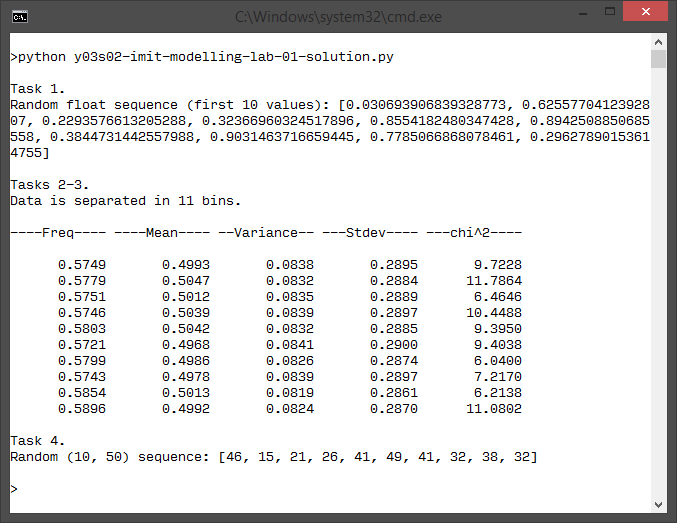
\includegraphics[height = 12\baselineskip]{./assets/y03s02-imitmod-lab-01-p01.png}
				\caption{Результат роботи програмної реалізації}
				\label{fig:res}
			\end{figure}

			Оцінимо якість розробленого генератора та~згенерованих послідовностей. Як~бачимо з~результату, було згенеровано 10~послідовностей. Отримані значення частотного тесту послідовностей близькі до~цільових значень еталонного генератора псевдовипадкових чисел~(розділ~\ref{sssec:freq-test}). 
			
			Розглянемо значення критерію Пірсона. Області значень випадкових чисел кожної послідовності були розділені на~$k = 11$~інтервалів, тому значення ступенів свободи~$v = k - 1 = 10$. Порівнюємо експериментальні значення з~теоретичними~(табл.~\ref{tab:chi-squared-values-per-df}) і~бачимо, що~отримані~$p$-значення близькі до~\SI{50}{\percent}, що~є показником якісного генератора.
			\begin{table}[!htbp]
				\centering
				\caption{Деякі значення~$\chi^{2}$-розподілу для ступенів свободи~$v = 10$}
				\label{tab:chi-squared-values-per-df}
				\begin{tabular}{
						v{2\gridunitwidth - 2\tabcolsep}
						n{2\gridunitwidth - 2\tabcolsep}
						n{2\gridunitwidth - 2\tabcolsep}
						n{2\gridunitwidth - 2\tabcolsep}
						n{2\gridunitwidth - 2\tabcolsep}
						n{2\gridunitwidth - 2\tabcolsep}
				}
					\toprule
						Ступені свободи~$v$ & $p = \SI{5}{\percent}$ & $p = \SI{25}{\percent}$ & $p = \SI{50}{\percent}$ & $p = \SI{75}{\percent}$ & $p = \SI{95}{\percent}$ \\ 
					\midrule
						10 & \num{3.940} & \num{6.737} & \num{9.342} & \num{12.550} & \num{18.310} \\ 
					\bottomrule
				\end{tabular}
			\end{table}

			Статистичні параметри згенерованих послідовностей також близькі до~параметрів еталонного генератора~(розділ~\ref{ssec:stat-params}). Отже, можемо зробити висновок, що~розроблена реалізація є~високоякісним лінійним конгруентним генератором псевдовипадкових чисел. 


	\section{Висновок}
		Виконуючи дану лабораторну роботу ми ознайомились з~еталоном функціонування генератора псевдовипадкових чисел; побудували імітаційну модель функціонування генератора псевдовипадкових чисел на~основі лінійного конгруентного методу та~здійснили перевірку якості роботи створеного генератора псевдовипадкових чисел.

		\appendix
		\section{Повний початковий код програмної реалізації}
		\label{sec:full-listing}
			\begin{listingpython}[toprule = 0pt, bottomrule = 0pt]{Повний початковий код програмної реалізації}{lst:full-solution}
#!/usr/bin/env python3

import random # random.SystemRandom() for generating seed
import math # math.sqrt
import numpy as np

BINS = 11
RANDMIN = 10
RANDMAX = 50

# A class implementing an LCG and relevant methods
class LCG:
    rand_seq = []

    # generator
    def lcg(self, m, a, c, seed):
        while True:
            seed = (a * seed + c) % m
            yield seed

    def __init__(self,
                 m = 0x7FFFFFFF, # modulus M (as per MINSTD), Mersenne 31, prime
                 a = 48271, # multiplier a, prime number
                 c = 0, # increment c
                 seed = random.SystemRandom().randint(0, 0xFFFFFFFF)):
        self.m, self.a, self.c, self.seed = m, a, c, seed
        self.rand_seq = self.lcg(self.m, self.a, self.c, self.seed)

    def randint(self):
        return next(self.rand_seq)

    def randfloat(self):
        return next(self.rand_seq) / self.m

def calc_freq(seq, a, b):
    cnt = 0
    for x in seq:
        if a < x < b:
            cnt += 1

    return cnt / len(seq)

def calc_mean(seq):
    return sum(seq) / len(seq)

def calc_variance(seq):
    if len(seq) == 1:
        return 0

    mean = calc_mean(seq)
    variance = sum([pow(x - mean, 2) for x in seq]) / len(seq)
    return variance

def calc_stdev(seq):
    return math.sqrt(calc_variance(seq))

def calc_stat_params(seq):
    return calc_mean(seq), calc_variance(seq), calc_stdev(seq)

def calc_chi_squared_pearson(seq):
    m = BINS
    N = len(seq)

    freqs = np.histogram(seq, bins = m)[0] # bin data in m bins

    return m/N * sum([pow( x - N/m, 2) for x in freqs])

def calc_seq_props(seq):
    freq = calc_freq(seq, 0.2113, 0.7887)
    mean = calc_mean(seq)
    variance = calc_variance(seq)
    stdev = calc_stdev(seq)
    chi_squared = calc_chi_squared_pearson(seq)

    return freq, mean, variance, stdev, chi_squared

def calc_all_seq_props(dataset):
    res = []
    for seq in dataset:
        res.append(calc_seq_props(seq))

    return res

def print_res(p):
    print('\n{:-^12} {:-^12} {:-^12} {:-^12} {:-^12}'.format('Freq', 'Mean', 'Variance', 'Stdev', 'chi^2'))
    print()
    for s in p:
        print('{:>12.4f} {:>12.4f} {:>12.4f} {:>12.4f} {:>12.4f}'.format(*s))

def build_rand_range(a, b, count = 10):
    res = []
    for i in range(count):
        res.append(random.randrange(a, b))

    return res


def main():
    lcg = LCG() # instantiate an LCG

    a, b = RANDMIN, RANDMAX # randint bounds

    rand_float_seqs = []
    rand_int_seq = build_rand_range(a, b)

    # build test sequence
    for i in range(10):
        seq = [lcg.randfloat() for x in range(10000)]
        rand_float_seqs.append(seq)

    print('\nTask 1.\nRandom float sequence (first 10 values): {}'.format(rand_float_seqs[0][:10]))

    print('\nTasks 2-3.\nData is separated in {} bins.'.format(BINS))

    properties = calc_all_seq_props(rand_float_seqs)
    print_res(properties)

    print('\nTask 4.\nRandom ({}, {}) sequence: {}'.format(a, b, rand_int_seq))


if __name__ == '__main__':
    main()
			\end{listingpython}

\end{document}

